\begin{mainquestion}{nodalpower}{Nodal Analysis}
Consider the following circuit.

\begin{center}
    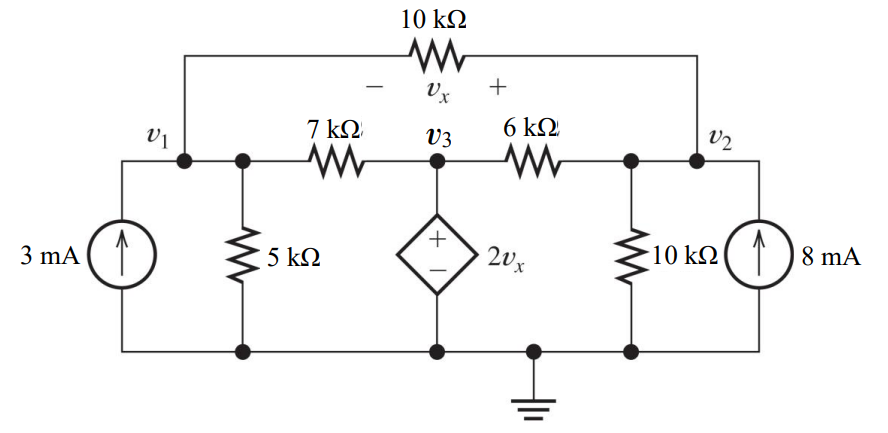
\includegraphics[width=0.8\textwidth]{schematic.png}
\end{center}

% =========================================================
\begin{partquestion}{nodal}
{Use nodal analysis to find each of the node voltages $v_1$, $v_2$ and $v_3$.}

\begin{answer}
We can leave out units, assuming all currents are \qty{}{\milli\ampere}, all resistances are \qty{}{\kilo\ohm} and all voltages are \qty{}{\volt}. Writing KCL using the nodal voltages at node 1 gives:
\begin{gather*}
\qty{3}{\milli\ampere}
=
\frac{v_1}{\qty{5}{\kilo\ohm}}
+
\frac{v_1 - v_2}{\qty{10}{\kilo\ohm}}
+
\frac{v_1 - v_3}{\qty{7}{\kilo\ohm}} \\
\qty{3}{\milli\ampere}
=
\frac{31}{70}v_1
-
\frac{1}{10}v_2
-
\frac{1}{7}v_3
\end{gather*}

Writing KCL using the nodal voltages at node 2 gives:
\begin{gather*}
\qty{8}{\milli\ampere}
=
\frac{v_2}{\qty{10}{\kilo\ohm}}
+
\frac{v_2 - v_1}{\qty{10}{\kilo\ohm}}
+
\frac{v_2 - v_3}{\qty{6}{\kilo\ohm}} \\
\qty{8}{\milli\ampere}
=
-\frac{1}{10}v_1
+
\frac{11}{30}v_2
-
\frac{1}{6}v_3
\end{gather*}

We can see that
\[
v_3 = 2v_x = 2(v_2 - v_1),
\]
so we can substitute this value into the two KCL equations above to get:

\begin{gather*}
\qty{3}{\milli\ampere}
=
\frac{31}{70}v_1
-
\frac{1}{10}v_2
-
\frac{2}{7}(v_2 - v_1)
=
\frac{51}{70}v_1
-
\frac{27}{70}v_2 \\
\qty{8}{\milli\ampere}
=
-\frac{1}{10}v_1
+
\frac{11}{30}v_2
-
\frac{1}{3}(v_2 - v_1)
=
\frac{7}{30}v_1
+
\frac{1}{30}v_2
\end{gather*}

This gives two equations and two unknowns. Multiply the bottom one by \(\frac{81}{7}\) and add them together to get:
\begin{align*}
3 + \frac{648}{7} &= (\frac{51}{70} + \frac{81}{7}\cdot\frac{7}{30})v_1 \\
\frac{669}{7} &= \frac{240}{70}v_1 \\
v_1 &= \frac{223}{8} = \qty{27.875}{\volt}
\end{align*}
And it follows that
\begin{align*}
3 &= \frac{51}{70} \cdot \frac{223}{8} - \frac{27}{70}v_2 \\
v_2 &= \frac{70}{27}(\frac{51}{70} \cdot \frac{223}{8} - \frac{1680}{560}) \\
v_2 &= \frac{70}{27}(\frac{9693}{560}) \\
v_2 &= \frac{359}{8} = \qty{44.875}{\volt}
\end{align*}

and
\[
v_3
=
2(v_2 - v_1)
=
2\left(\frac{359}{8} - \frac{223}{8}\right)
=
\qty{34}{\volt}.
\]
\end{answer}
\end{partquestion}

% =========================================================
\begin{partquestion}{findx}
{Find $v_x$}

\begin{answer}
\[
v_x = \frac{1}{2}v_3
= \frac{1}{2}\left(\qty{34}{\volt}\right)
= \qty{17}{\volt}.
\]
\end{answer}
\end{partquestion}

% =========================================================
\begin{partquestion}{branch}
{Find the 8 branch currents $i_k$, where $k$ takes on values 1 through 8 (ordered by element position in circuit, from top to bottom, left to right)}

\begin{answer}
Assuming the branch current is defined as flowing from right to left (Passive Sign Convention):

\begin{align}
i_1 &= \frac{v_2 - v_1}{\qty{10}{\kilo\ohm}} = \qty{1.7}{\milli\ampere} \\
i_2 &= \frac{v_3 - v_1}{\qty{7}{\kilo\ohm}} = \qty{0.875}{\milli\ampere} \\
i_3 &= \frac{v_2 - v_3}{\qty{6}{\kilo\ohm}} = \qty{1.8125}{\milli\ampere} \\
i_4 &= \qty{-3}{\milli\ampere} \\
i_5 &= \frac{v_1}{\qty{5}{\kilo\ohm}} = \qty{5.575}{\milli\ampere} \\
i_6 &= i_3 - i_2 = \qty{0.9375}{\milli\ampere} \\
i_7 &= \frac{v_2}{\qty{10}{\kilo\ohm}} = \qty{4.4875}{\milli\ampere} \\
i_8 &= \qty{-8}{\milli\ampere}
\end{align}
\end{answer}
\end{partquestion}

% =========================================================
\begin{partquestion}{power}
{What is the power dissipated in the circuit?}

\begin{answer}
The power dissipated is the sum of the positive product $VI$ for each element. This includes the resistors and the dependent voltage source since the current is positive when flowing from $+$ to $-$.

\begin{align*}
P_{\text{diss}} &= (v_2 - v_1)i_1 + (v_3 - v_1)i_2 + (v_2 - v_3)i_3 + v_1i_5 + v_3i_6 + v_2i_7 \\
&= (17)(1.7) + (6.125)(0.875) + (10.875)(1.8125) \\
&\hspace{1cm} + (27.875)(5.575) + (34)(0.9375) + (44.875)(4.4875) \\
&\approx \qty{443}{\milli\watt}
\end{align*}

\end{answer}
\end{partquestion}

% =========================================================
\begin{partquestion}{tellegen}
{What is the total power in the circuit?}

\begin{answer}
By Tellegen’s theorem, the total power in the circuit must be zero. This means that the two independent sources should be supplying \qty{443}{\milli\watt} of power. We can check this:

\begin{align*}
P_{\text{diss}} &= -v_1i_4 + v_2i_8\\
&= -(27.875)(-3) - (44.875)(-8) \\
&\approx \qty{443}{\milli\watt}
\end{align*}

so everything is indeed copacetic.
\end{answer}
\end{partquestion}

\end{mainquestion}